\section{\texorpdfstring{Sériová komunikace}{Seriova komunikace}}

% =====================================================================================================================
	\begin{frame}
    \frametitle{Sériová komunikace}
    
    \begin{itemize}
      \item způsob přenosu dat, při kterém se informace posílají postupně po jednotlivých bitech za sebou,
      \item jako komunikační kanál v jednom směru často dostačuje jen jeden vodič.
    \end{itemize}
    
    \vspace{5mm}
    \textbf{Základní princip:}
    
    \begin{itemize}
      \item Odeslání binární hodnoty $(10110010)_2$,
      \item na komunikační kanál vysílač postupně se stanovenou periodou zadává hodnoty:
      \begin{center}
        $1 \longrightarrow 0 \longrightarrow 1 \longrightarrow 1 \longrightarrow 0 \longrightarrow 0 \longrightarrow 1 \longrightarrow 0$
      \end{center}
      \item \textcolor{red}{přijímač i vysílač musí nějakým způsobem stanovit časový interval pro vyslání a čtení hodnoty v komunikačním kanálu.}
    \end{itemize}

	\end{frame}
  
% =====================================================================================================================
	\begin{frame}
    \frametitle{Sériová komunikace - výhody}
    
    \begin{itemize}
      \item méně vodičů,
      \item jednodušší zapojení,
      \item levnější hardware,
      \item možnost komunikace na větší vzdálenosti,
      \item menší citlivost na rušení.
    \end{itemize}
    
    Poslední dva body platí především pro linky využívající proudovou smyčku nebo diferenciální pár.
    
    \vspace{3mm}
    \textbf{Rozlišujeme:}
    
    \begin{itemize}
      \item \textcolor{blue}{\textbf{synchronní}} komunikaci - zařízení sdílí společný hodinový signál (SPI, I\textsuperscript{2}C),
      \item \textcolor{blue}{\textbf{asynchronní}} komunikaci - bez sdíleného hodinového signálu (RS232, RS485).
    \end{itemize}
	\end{frame}

% =====================================================================================================================
	\begin{frame}
    \frametitle{SPI}
    
		\textbf{\textcolor{blue}{S}erial \textcolor{blue}{P}eripheral \textcolor{blue}{I}nterface}
    
    \begin{itemize}
      \item komunikace s paměťmi a senzory,
      \item jeden obvod je řídicí - Master a vystavuje řídicí signály komunikace,
      \item ostatní obvody, jsou typu Slave,
      \item Full-Duplex komunikace - oběma směry se komunikuje v jeden moment,
      \item je určena pro kratší komunikační vzdálenosti,
      \item čtení i vyslání bitu je řízeno hodinovým signálem, který je součástí komunikace,
      \item rychlost komunikace definuje Master pomocí hodinového signálu a je omezena jen fyzikálními limity komunikační linky.
    \end{itemize}

	\end{frame}
  
% =====================================================================================================================
	\begin{frame}
    \frametitle{SPI - zapojení}
    
    \begin{center}
      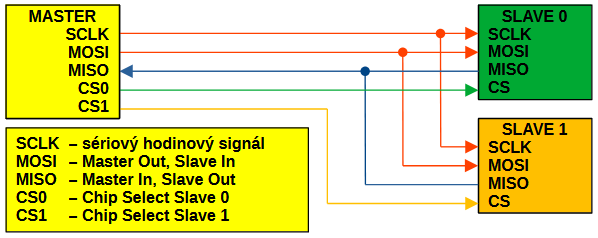
\includegraphics[width=0.90\textwidth]{fig/SPI.png}
    \end{center}
    
    
    \begin{itemize}
      \item Lze komunikovat s více Slave jednotkami na jedné sběrnici, pokud existuje příslušný CS signál.
    \end{itemize}

	\end{frame}
  
  
 % =====================================================================================================================
	\begin{frame}
    \frametitle{SPI - CPHA = 0}
    
    \begin{center}
      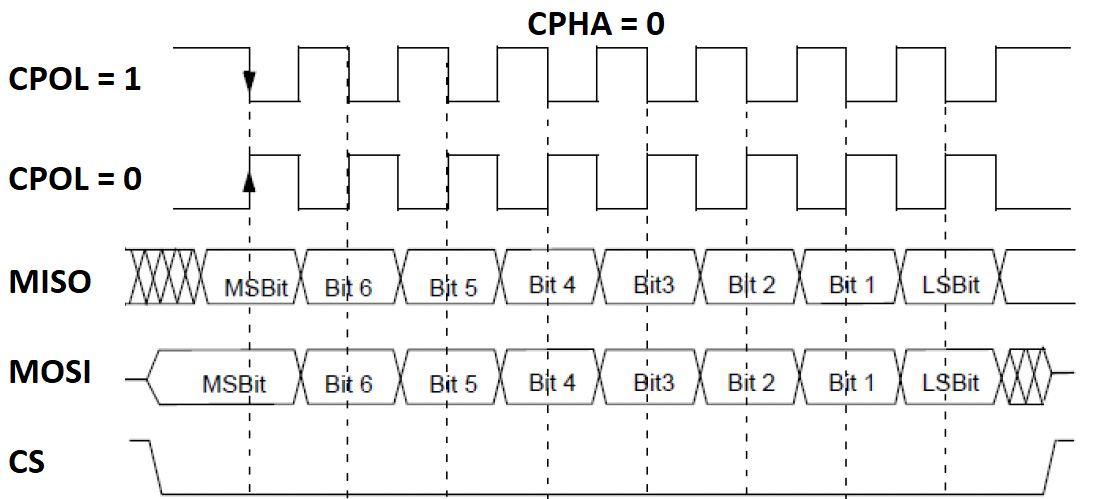
\includegraphics[width=0.90\textwidth]{fig/SPIModeCPHA0.png}
    \end{center}
    
    \begin{itemize}
      \item Čtení signálu při přechodu z \textcolor{blue}{\textbf{neaktivního do aktivního}} stavu hodin = \textcolor{blue}{\textbf{lichá hrana}},
      \item neaktivní stav je přímo dán stavem CPOL.
    \end{itemize}

	\end{frame}
 
 % =====================================================================================================================
	\begin{frame}
    \frametitle{SPI - CPHA = 1}
    
    \begin{center}
      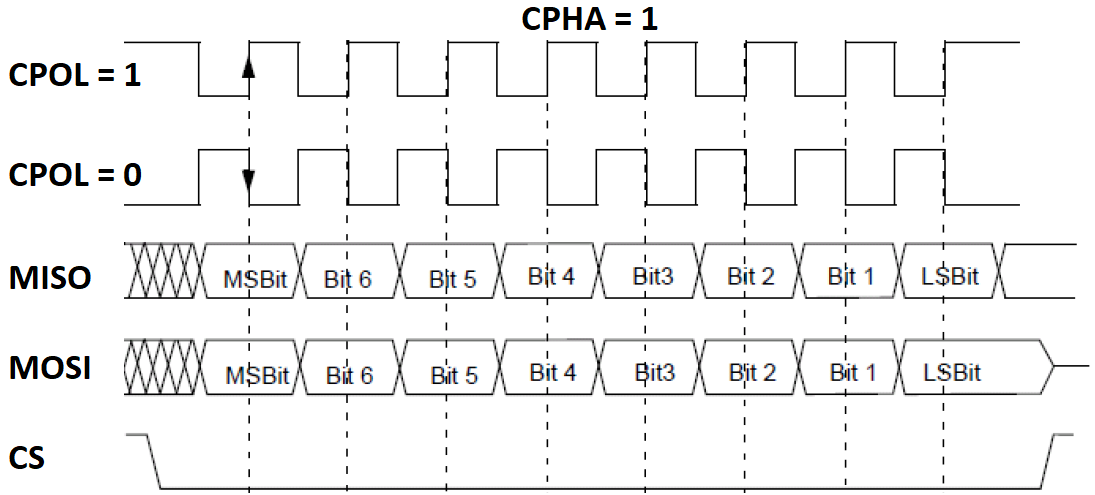
\includegraphics[width=0.90\textwidth]{fig/SPIModeCPHA1.png}
    \end{center}
    
    \begin{itemize}
      \item Čtení signálu při přechodu z \textcolor{blue}{\textbf{aktivního do neaktivního}} stavu hodin = \textcolor{blue}{\textbf{sudá hrana}},
      \item neaktivní stav je přímo dán stavem CPOL.
    \end{itemize}

	\end{frame}
  
% =====================================================================================================================
	\begin{frame}
    \frametitle{SPI - ukázka, loopback}
    
    \begin{minipage}[t][\textheight][t]{0.3\textwidth}
      \textbf{Zapojení:}
      
      \begin{center}
        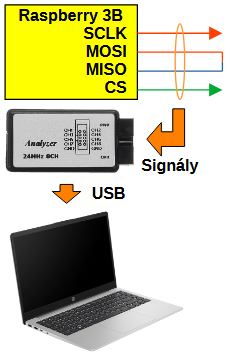
\includegraphics[width=1.00\textwidth]{fig/spirpi.png}
      \end{center}
      
		\end{minipage}
		\begin{minipage}[t][\textheight][t]{0.65\textwidth}
      \textbf{RPI program:}
      
      \begin{center}
        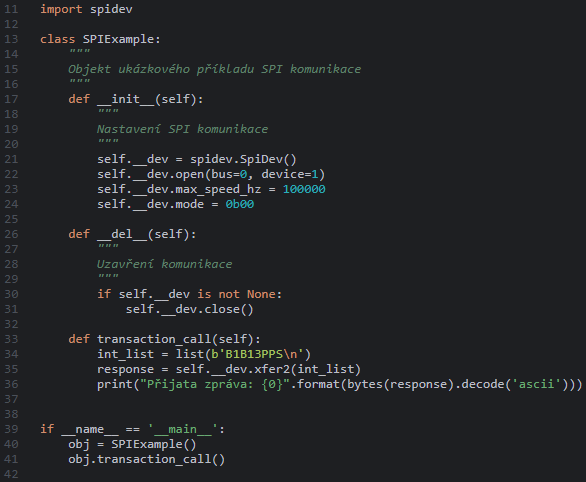
\includegraphics[width=1.00\textwidth]{fig/spirpipython.png}
      \end{center}
      
		\end{minipage}

	\end{frame}
  
% =====================================================================================================================
	\begin{frame}
    \frametitle{SPI - logický analyzátor}
    
    \begin{center}
      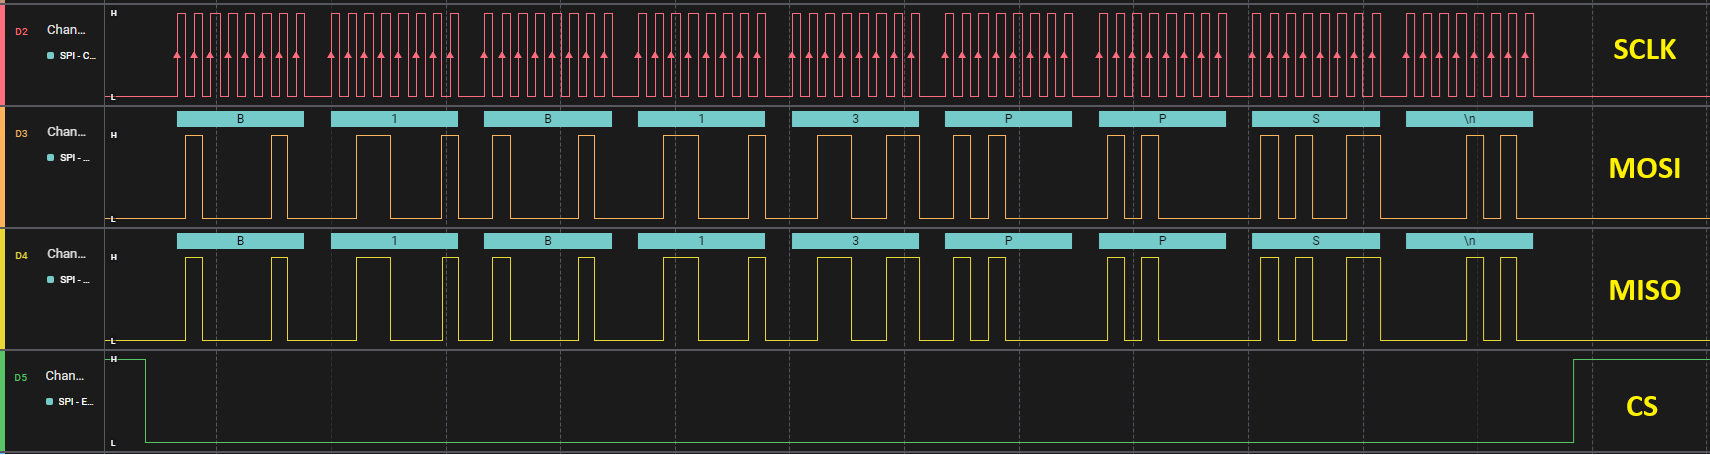
\includegraphics[width=1.00\textwidth]{fig/SPIExample.png}
    \end{center}
    
    
    \begin{itemize}
      \item Znaky jsou kódovány pomocí ASCII,
      \item CPOL=0, klidová hodnota hodin je 0
      \item CPHA=0, lichá hrana, přechod z 0 do 1
    \end{itemize}

	\end{frame}

% =====================================================================================================================
	\begin{frame}
    \frametitle{ASCII tabulka}
    
    \begin{center}
      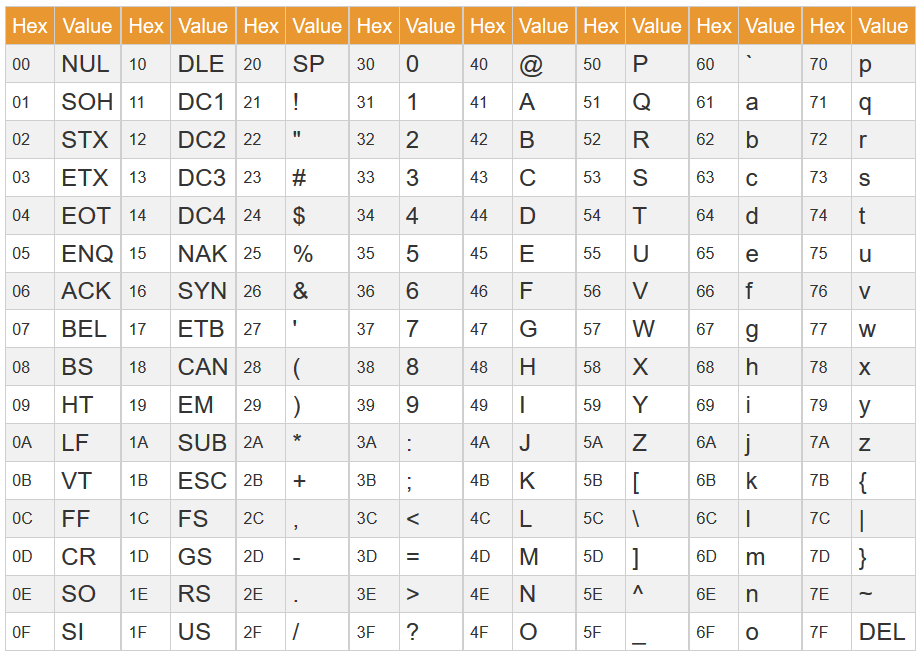
\includegraphics[width=0.85\textwidth]{fig/ascii-table.png}
    \end{center}

	\end{frame}

% =====================================================================================================================
	\begin{frame}
    \frametitle{UART}
    
    \textbf{\textcolor{blue}{U}niversal \textcolor{blue}{A}synchronous \textcolor{blue}{R}eceiver-\textcolor{blue}{T}ransmitter}
    
    \begin{itemize}
      \item Základ pro:
      
      \begin{itemize}
        \item standard RS232, RS422: komunikace mezi dvěma rovnocennými zařízeními,
        \item standard RS485: komunikace mezi mnoha zařízeními (\textcolor{blue}{Half-Duplex})
      \end{itemize}
      
      \item počátky v 60. letech (1969 RS232C), 
      \item formát se stále používá v průmyslu - Modbus RTU, M-Bus, ...
      \item základem je obousměrná komunikace po 2/3 vodičích,
      \item RS232 používá navíc řídicí vodiče RTS, CTS, DTR, RI, DCD,
      \item standardy se liší v napěťových úrovních:
      
      \begin{itemize}
        \item \textbf{RS232:} log. \textbf{0}: -15V až -3V, log. \textbf{1}: 3V až 15V
        \item \textbf{TTL:} log. \textbf{0}: 0V, log. \textbf{1}: 5V
      \end{itemize}
    \end{itemize}

	\end{frame}
  
% =====================================================================================================================
	\begin{frame}
    \frametitle{UART - zapojení}
    
    \begin{center}
      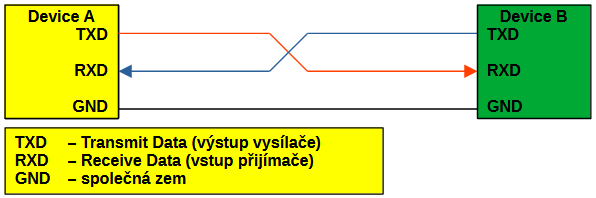
\includegraphics[width=0.90\textwidth]{fig/UART.png}
    \end{center}
    
    \begin{itemize}
      \item Bez vodiče sdíleného hodinového signálu:
      
      \begin{itemize}
        \item musí dojít k synchronizaci přijímače s vysílanými daty,
        \item se musí shodovat přenosová rychlost,
        \item se musí shodovat rámec přenášených dat (např. počet bitů).
      \end{itemize}
    \end{itemize}
	\end{frame}
  
% =====================================================================================================================
	\begin{frame}
    \frametitle{UART - datový rámec}
    
    \textbf{Rámec pro 8 datových bitů, 1 stop bit a bez parity:}
    \begin{center}
      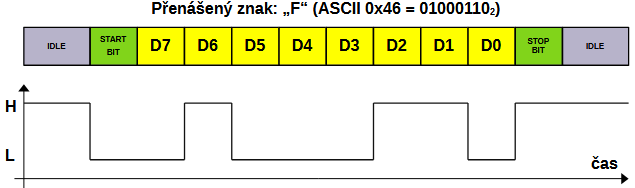
\includegraphics[width=0.90\textwidth]{fig/uartframe.png}
    \end{center}
    
    \begin{center}
      \begin{tabular}{| l | l |}
        \hline
        \textbf{START BIT} & Označuje začátek rámce - hrana \\
        \hline
        \textbf{D7:0} & Data, pořadí \textbf{MSB}$\rightarrow$\textbf{LSB} \\
        \hline
        \textbf{STOP BIT} & Linka je v klidové úrovni po dobu 1 bitu \\
        \hline
      \end{tabular}
    \end{center}
    
	\end{frame}

% =====================================================================================================================
	\begin{frame}
    \frametitle{UART - vlastnosti}
    \small
    \begin{itemize}
      \item \textbf{Baud (Bd)}: jednotka modulační rychlosti, počet změn stavu přenosového média za sekundu,
      \item standardizované rychlosti: 150, 300, 600, 1200, 2400, 4800, 9600, 19200, 38400, 57600 a 115200 Bd
      \item vždy 1 start bit,
      \item pořadí dat:
      
      \begin{itemize}
        \item \textbf{MSB}$\rightarrow$\textbf{LSB}
        \item \textbf{LSB}$\rightarrow$\textbf{MSB}
      \end{itemize}
      
      \item možnost paritního bitu:
      
      \begin{itemize}
        \item sudá parita doplňuje počet 1 na sudý počet,
        \item lichá parita doplňuje počet jedniček na lichý počet,
      \end{itemize}
      
      \item 1, 1.5 nebo 2 stop bity.
      
    \end{itemize}
    
	\end{frame}
  
% =====================================================================================================================
	\begin{frame}
    \frametitle{UART - ukázka, loopback}
    
    \begin{minipage}[t][\textheight][t]{0.3\textwidth}
      \textbf{Zapojení:}
      
      \begin{center}
        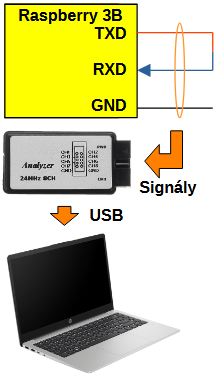
\includegraphics[width=0.97\textwidth]{fig/uartrpi.png}
      \end{center}
      
		\end{minipage}
		\begin{minipage}[t][\textheight][t]{0.65\textwidth}
      \textbf{RPI program:}
      
      \begin{center}
        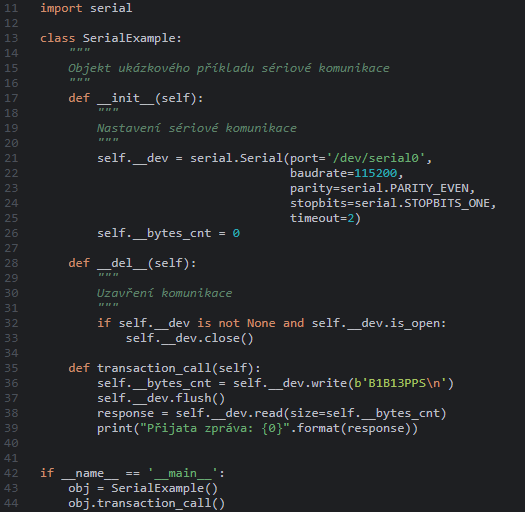
\includegraphics[width=0.85\textwidth]{fig/uartrpipython.png}
      \end{center}
      
		\end{minipage}

	\end{frame}
  
% =====================================================================================================================
	\begin{frame}
    \frametitle{UART - logický analyzátor}
    
    \begin{center}
      \includegraphics[width=1.00\textwidth]{fig/SerialExample.png}
    \end{center}
    
    
    \begin{itemize}
      \item Jednodušší komunikace než SPI,
      \item formát přenosu musí být nastaven dopředu na obou stranách.
    \end{itemize}

	\end{frame}